\documentclass[12pt, a4paper]{article}
\usepackage{polski}
\usepackage[utf8]{inputenc}       	% nadaje dokumentowi polską składnię
\usepackage{geometry}
\usepackage{graphicx}
\usepackage{amsmath}
\usepackage{listings}
\usepackage{color}
\usepackage[colorlinks=true, urlcolor=blue]{hyperref}
%\usepackage[draft]{graphicx}
\usepackage{listings}
\definecolor{mygreen}{rgb}{0,0.6,0}
\definecolor{mygray}{rgb}{0.5,0.5,0.5}
\definecolor{mymauve}{rgb}{0.58,0,0.82}


\lstset{ %
	backgroundcolor=\color{white},   % choose the background color; you must add \usepackage{color} or \usepackage{xcolor}; should come as last argument
	basicstyle=\footnotesize,        % the size of the fonts that are used for the code
	breakatwhitespace=false,         % sets if automatic breaks should only happen at whitespace
	breaklines=true,                 % sets automatic line breaking
	captionpos=b,                    % sets the caption-position to bottom
	commentstyle=\color{mygreen},    % comment style
	deletekeywords={...},            % if you want to delete keywords from the given language
	escapeinside={\%*}{*)},          % if you want to add LaTeX within your code
	extendedchars=true,              % lets you use non-ASCII characters; for 8-bits encodings only, does not work with UTF-8
	frame=single,	                   % adds a frame around the code
	keepspaces=true,                 % keeps spaces in text, useful for keeping indentation of code (possibly needs columns=flexible)
	keywordstyle=\color{blue},       % keyword style
	language=Octave,                 % the language of the code
	morekeywords={*,...},            % if you want to add more keywords to the set
	numbers=left,                    % where to put the line-numbers; possible values are (none, left, right)
	numbersep=5pt,                   % how far the line-numbers are from the code
	numberstyle=\tiny\color{mygray}, % the style that is used for the line-numbers
	rulecolor=\color{black},         % if not set, the frame-color may be changed on line-breaks within not-black text (e.g. comments (green here))
	showspaces=false,                % show spaces everywhere adding particular underscores; it overrides 'showstringspaces'
	showstringspaces=false,          % underline spaces within strings only
	showtabs=false,                  % show tabs within strings adding particular underscores
	stepnumber=1,                    % the step between two line-numbers. If it's 1, each line will be numbered
	stringstyle=\color{mymauve},     % string literal style
	tabsize=2,	                   % sets default tabsize to 2 spaces
	title=\lstname                   % show the filename of files included with \lstinputlisting; also try caption instead of title
}

\newcommand{\myparagraph}[1]{\paragraph{#1}\mbox{}\\}
\begin{document}
	\begin{titlepage}
		\newgeometry{top=5cm}
		\centering
		\vfill
		{\bfseries\Large
			Metody Obliczeniowe w Nauce i Technice\\
			Laboratorium\\
			Sprawozdanie z ćwiczenia
			\vskip2cm
			Marcin Maleńczuk\\
		}    
		\vfill
		
\includegraphics[width=4cm]{logo.jpg}
		\vfill
		\vfill
	\end{titlepage}
	\newgeometry{tmargin=1.5cm, bmargin=1.5cm, lmargin=1cm, rmargin=1cm} 
\section{Dane}
\begin{lstlisting}[caption={Węzły Interpolacji},language=R,label={lst:data}]
	X = LinRange(-1, 1, 10)
	Y = [rand() for x in X]
	xsf = LinRange(-1, 1, 1000)
	xs = LinRange(1, length(X), 1000)
	
	scatter(X, Y, label="Nodes", title="Interpolation nodes")
\end{lstlisting}
Listing~\ref{lst:data} generuje 10 węzłów interpolacji
\begin{figure}[ht!]
	\centering    
	\def\svgwidth{\columnwidth}
	\input{Interpolation_nodes.pdf_tex}
	\caption{Węzły Interpolacji}
	\label{fig:data}
\end{figure}
\clearpage
\section{Lagrange}}
\begin{lstlisting}[caption={Interpolacja Lagrange'a},language=R,label={lst:lagrange}]
function lagrange(X::AbstractArray, Y::AbstractArray, x::Number)
	k = length(X)
	return sum([reduce(*, [(x - X[m])/(X[j] - X[m]) for m in 1:k if m != j]) * Y[j] for j in 1:k])
end

function lagrange(X::AbstractArray, Y::AbstractArray, xx::AbstractArray)
	return [lagrange(X, Y, x) for x in xx]
end

LY = lagrange(X, Y, xsf)
scatter(X, Y, label="Nodes", title = "Lagrange interpolation")
plot!(xsf, LY, label = "Lagrange")
\end{lstlisting}
Listing~\ref{lst:lagrange} wykonuję na węzłach wygenerowanych z Listing~\ref{lst:data} interpolację wielomianową Lagrange'a
\begin{figure}[ht!]
	\centering    
	\def\svgwidth{\columnwidth}
	\input{Lagrange_interpolation.pdf_tex}
	\caption{Interpolacja Lagrange'a}
	\label{fig:Lagrange}
\end{figure}
\clearpage
\section{Newton}
\begin{lstlisting}[caption={Interpolacja Newton'a},language=R,label={lst:newton}]
function divdif(X::AbstractArray, Y::AbstractArray)
	n = length(X)
	d = convert(Array{Float64,1}, deepcopy(Y))
	for i=2:n
		for j=1:i-1
			d[i] = (d[j] - d[i])/(X[j] - X[i])
		end
	end
	return d
end

function newtonform(X::AbstractArray, d::AbstractArray, x::Number) 
	n = length(d)
	result = d[n]
	for i=n-1:-1:1
		result = result * (x - X[i]) + d[i]
	end
	return result
end

function newton(X::AbstractArray, Y::AbstractArray, x::Number)
	divided = divdif(X, Y)
	result = newtonform(X, divided, x)
	return result
end

function newton(X::AbstractArray, Y::AbstractArray, xx::AbstractArray)
	divided = divdif(X, Y)
	results = [newtonform(X, divided, x) for x in xx]
	return results
end

NY = newton(X, Y, xsf)
scatter(X, Y, label="Nodes", title = "Newton interpolation")
plot!(xsf, NY, label = "Newton")
\end{lstlisting}
Listing~\ref{lst:newton} wykonuję na węzłach wygenerowanych z Listing~\ref{lst:data} interpolację wielomianową Newton'a
\begin{figure}[ht!]
	\centering    
	\def\svgwidth{\columnwidth}
	\input{Newton_interpolation.pdf_tex}
	\caption{Interpolacja Newtona'a}
	\label{fig:newton}
\end{figure}
\clearpage
\section{Polynomials}
\begin{lstlisting}[caption={Interpolacja pakietu Polynomials},language=R,label={lst:polynomials}]
poly = polyfit(X, Y, length(X) - 1)
PY = polyval(poly, xsf)
scatter(X, Y, label="Nodes", title = "Polynomials interpolation")
plot!(xsf, PY, label = "Polynomials")
\end{lstlisting}
Listing~\ref{lst:polynomials} wykonuję na węzłach wygenerowanych z Listing~\ref{lst:data} interpolację wielomianową dostępną w pakiecie Polynomials
\begin{figure}[ht!]
	\centering    
	\def\svgwidth{\columnwidth}
	\input{Polynomials_interpolation.pdf_tex}
	\caption{Interpolacja pakietu Polynomials}
	\label{fig:olynomials}
\end{figure}
\clearpage
\section{Porównanie Interpolacji}
\begin{lstlisting}[caption={Porównanie Interpolacji},language=R,label={lst:comparison}]
scatter(X, Y, label="Nodes", title = "Interpolation comparison")
plot!(xsf, LY, label = "Lagrange")
plot!(xsf, NY, label = "Newton")
plot!(xsf, PY, label = "Polynomials")
\end{lstlisting}
Listing~\ref{lst:polynomials} nanosi na Rysunek~\ref{fig:comparison} poprzednie interpolację wielomianowe.
Na Rysunek~\ref{fig:comparison} widać że wszystkie interpolacje wilomianowe dają ten sam wielomian. Wynika to z twierdzenia o Jednoznaczności wielomianu interpolacyjnego, które mówi że dla danych węzłów interpolacji istnieje tylko jeden wielomian który je interpoluje.
\begin{figure}[ht!]
	\centering    
	\def\svgwidth{\columnwidth}
	\input{Interpolation_comparison.pdf_tex}
	\caption{Porównanie Interpolacji}
	\label{fig:comparison}
\end{figure}
\begin{lstlisting}[caption={Porównanie szybkości Interpolacji},language=R,label={lst:time_comparison}]
function times()
	df = DataFrame(Knots = Int64[], Fun = String[], Time = Float64[])
	for l in 10:10:250
		for i in 1:10
			x = LinRange(-1, 1, l)
			y = [rand() for _ in x]
			push!(df, [l, "Polynomials", (@elapsed polyval(polyfit(x, y, length(x) - 1), x))])
			push!(df, [l, "Newton", (@elapsed newton(x, y, x))])
			push!(df, [l, "Lagrange", (@elapsed lagrange(x, y, x))])
		end
	end
	return df
end

d = aggregate(times(), [:Knots, :Fun], [mean, std])
s = scatter(d[:Knots], 
	d[:Time_mean], 
	group = d[:Fun], 
	yerr = d[:Time_std], 
	legend = :topleft,
	title = "Interpolation time comparison",
	ylabel = "time [s]", 
	xlabel = "knots")
\end{lstlisting}
Listing~\ref{fig:time_comparison} porównuję czasy wykonania dla poszczególnych interpolacji zaczynając od 10 węzłów a kończąc na 250 co 10.
Na Rysunek~\ref{fig:time_comparison} widać, że czas interpolacji wielomianem Lagrange'a rośnie znacznie szybciej niż wilemoaniam Newton'a dlatego nie jest ona używana tylko do dowdów.
\begin{figure}[ht!]
	\centering    
	\def\svgwidth{\columnwidth}
	\input{Interpolation_time_comparison.pdf_tex}
	\caption{Porównanie szybkości Interpolacji}
	\label{fig:time_comparison}
\end{figure}
\clearpage
\section{Funkcje Sklejane}
\begin{lstlisting}[caption={Interpolacja funkcją sklejaną stopnia 1},language=R,label={lst:linear}]
litp = interpolate(Y, BSpline(Linear()))
L = litp(xs)
scatter(X, Y, label="Nodes", title = "BSpline linear interpolation")
plot!(xsf, L, label="BSpline linear")
\end{lstlisting}
Listing~\ref{lst:linear} wykonuję na węzłach wygenerowanych z Listing~\ref{lst:data} interpolację funkcjami sklejanymi stopnia pierwszego
\begin{figure}[ht!]
	\centering    
	\def\svgwidth{\columnwidth}
	\input{BSpline_linear_interpolation.pdf_tex}
	\caption{Interpolacja funkcją sklejaną stopnia 1}
	\label{fig:linear}
\end{figure}
\clearpage
\begin{lstlisting}[caption={Interpolacja funkcją sklejaną stopnia 2},language=R,label={lst:cubic}]
citp = interpolate(Y, BSpline(Cubic(Line(OnGrid()))))
C = citp(LinRange(1, length(X), 1000))
scatter(X,Y, label="Nodes", title = "BSpline cubic interpolation")
plot!(xsf,C, label="BSpline cubic")
\end{lstlisting}
Listing~\ref{lst:cubic} wykonuję na węzłach wygenerowanych z Listing~\ref{lst:data} interpolację funkcjami sklejanymi stopnia drugiego
\begin{figure}[ht!]
	\centering    
	\def\svgwidth{\columnwidth}
	\input{BSpline_cubic_interpolation.pdf_tex}
	\caption{Interpolacja funkcją sklejaną stopnia 2}
	\label{fig:cubic}
\end{figure}
\clearpage
\begin{lstlisting}[caption={Interpolacja funkcją sklejaną stopnia 3},language=R,label={lst:quadratic}]
qitp = interpolate(Y, BSpline(Quadratic(Line(OnCell()))))
Q = qitp(LinRange(1, length(X), 1000))
scatter(X,Y, label="Nodes", title = "BSpline quadratic interpolation")
plot!(xsf,Q, label="BSpline quadratic")
\end{lstlisting}
Listing~\ref{lst:quadratic} wykonuję na węzłach wygenerowanych z Listing~\ref{lst:data} interpolację funkcjami sklejanymi stopnia trzeciego
\begin{figure}[ht!]
	\centering    
	\def\svgwidth{\columnwidth}
	\input{BSpline_quadratic_interpolation.pdf_tex}
	\caption{Interpolacja funkcją sklejaną stopnia 3}
	\label{fig:quadratic}
\end{figure}
\clearpage
\begin{lstlisting}[caption={Porównanie interpolacji funkcjami sklejanymi do interpolacji wielomianem},language=R,label={lst:cmp}]
scatter(X,Y, label="Nodes", title = "BSpline interpolation comparison")
plot!(xsf, L, label="BSpline linear")
plot!(xsf,C, label="BSpline cubic")
plot!(xsf,Q, label="BSpline quadratic")
plot!(xsf, PY, label = "Polynomials")
\end{lstlisting}
Rysunek~\ref{fig:cmp} przedstawia porówanie interpolacji wielomanowej z interpolacją funkcjami sklejanymi. Na krańcach przedziału można zauważyć, że dla funkcji sklejanych nie występuję efekt Rungego w przeciwieństwie do wielomanu intepolacyjnego.
\begin{figure}[ht!]
	\centering    
	\def\svgwidth{\columnwidth}
	\input{BSpline_Polynomials_interpolation_comparison.pdf_tex}
	\caption{Porównanie interpolacji funkcjami sklejanymi do interpolacji wielomianem}
	\label{fig:cmp}
\end{figure}
\clearpage
\section{Efekt Rungego}
\begin{lstlisting}[caption={Efekt Rungego},language=R,label={lst:runge}]
runge(x) = 1/(1+25*x^2)

i = 5
p = plot(xsf, map(runge, xsf), label = "Runge function",title = string("Runge's phenomenon (Nodes = ", i, ""))
RX = LinRange(-1, 1, i)
RY = map(runge, RX)
scatter!(RX, RY, label = "Nodes")

rpoly = polyfit(RX, RY, length(RX) - 1)
R = polyval(rpoly, xsf)
plot!(xsf, R, label = "Intepolation")
\end{lstlisting}
Listing~\ref{lst:runge} interpoluję wielomianem funkecję Rungego w i równoodległych węzłach. Rysunek~\ref{fig:runge5},  Rysunek~\ref{fig:runge9} i Rysunek~\ref{fig:runge13} przedstwiają funkję Rungego wraz z coraz to większą ilością węzłów intepolacji oraz wielomianem je interpolującym. Wraz ze wzrostem węzłów można zauważyć coraz większy błąd interpolacji wielomianem na końcach przedziałow.
\begin{figure}[ht!]
	\centering    
	\def\svgwidth{\columnwidth}
	\input{Runge5.pdf_tex}
	\caption{Interpolacja wielomianem 4 stopmnia funkcji Rungego}
	\label{fig:runge5}
\end{figure}
\begin{figure}[ht!]  
	\def\svgwidth{\columnwidth}
	\input{Runge9.pdf_tex}
	\caption{Interpolacja wielomianem 8 stopmnia funkcji Rungego}
	\label{fig:runge9}
\end{figure}
\begin{figure}[ht!]
	\centering    
	\def\svgwidth{\columnwidth}
	\input{Runge13.pdf_tex}
	\caption{Interpolacja wielomianem 12 stopmnia funkcji Rungego}
	\label{fig:runge13}
\end{figure}
\clearpage
\section{Interpolacja w Grafice komputerowej}
\begin{lstlisting}[caption={Original Image},language=R,label={lst:original}]
img = rand(Float32, 5, 5)
f = heatmap(img, title = "Original")
scatter!(repeat(1:5,1, 5), transpose(repeat(1:5,1, 5)), legend=false, color = :white)
\end{lstlisting}
Listing~\ref{lst:original} tworzy macierz 5x5 z randomowymi wartościami. Zakładamy że jest to nasz obrazek początkowy.
\begin{figure}[ht!]
	\centering    
	\def\svgwidth{\columnwidth}
	\input{Original.pdf_tex}
	\caption{Orginal Image}
	\label{fig:original}
\end{figure}
\begin{figure}[ht!]
	\centering
	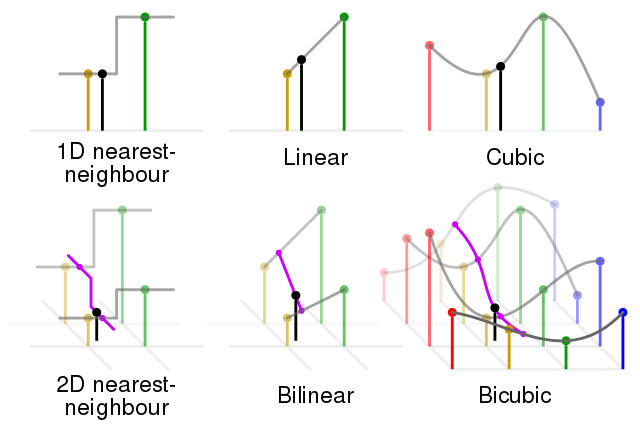
\includegraphics[scale=0.]{2dInterpolation.png}
	\caption{Comparison of some 1- and 2-dimensional interpolations} 
	\label{fig:2dInterpolation}      
\end{figure}
\clearpage
\begin{lstlisting}[caption={Interpolacja nearest},language=R,label={lst:nearest}]
function nearest(A::Matrix, xfactor::Number, yfactor::Number)
	lx, ly = size(A)
	nx, ny = round.(Int, (xfactor * lx, yfactor * ly))
	vx, vy = LinRange(0.5, lx + 0.5, nx), LinRange(0.5, ly+0.5, ny)
	itp = interpolate(A, BSpline(Constant()))
	etpf = extrapolate(itp, Flat())
	return etpf(collect(vx), collect(vy))
end

scale = 25
f = heatmap(nearest(img, scale, scale), title = "Nearest")
scatter!(repeat(1:5,1, 5)*scale-fill(scale/2,5,5), transpose(repeat(1:5,1, 5)*scale-fill(scale/2,5,5)), legend=false, color = :white)
\end{lstlisting}
Listing~\ref{lst:nearest} skaluje obrazek 25 krotnie stworzony w Listing~\ref{lst:original} korzystając z interpolacji nearest neighbor. Jest to metoda najprostsza, w której przy skalowaniu odbywa się wierne kopiowanie najbliższego piksela Rysunek~\ref{fig:2dInterpolation}. Metoda wymagająca od komputera najmniejszej mocy obliczeniowej, jednak jest rzadko stosowana, ponieważ w przypadku dużych powiększeń wyraźnie widać grupy identycznych pikseli, a granice pomiędzy nimi są wyraźne, ostre, nie rozmyte.
\begin{figure}[ht!]
	\centering    
	\def\svgwidth{\columnwidth}
	\input{Nearest.pdf_tex}
	\caption{Interpolacja nearest}
	\label{fig:nearest}
\end{figure}
\clearpage
\begin{lstlisting}[caption={Interpolacja bilinear},language=R,label={lst:bilinear}]
function bilinear(A::Matrix, xfactor::Number, yfactor::Number)
	lx, ly = size(A)
	nx, ny = round.(Int,  (xfactor * lx, yfactor * ly))
	vx, vy = LinRange(0.5, lx + 0.5, nx), LinRange(0.5, ly+0.5, ny)
	itp = interpolate(A, BSpline(Linear()))
	etpf = extrapolate(itp, Flat())
	return etpf(collect(vx), collect(vy))
end

scale = 25
f = heatmap(bilinear(img, 25, 25), title = "Bilinear")
scatter!(repeat(1:5,1, 5)*scale-fill(scale/2,5,5), transpose(repeat(1:5,1, 5)*scale-fill(scale/2,5,5)), legend=false, color = :white)
\end{lstlisting}
Listing~\ref{lst:bilinear} skaluje obrazek 25 krotnie stworzony w Listing~\ref{lst:original} korzystając z interpolacji bilinear. Jest to   metoda pośrednia, niewiele mocniej obciążająca komputer, ale i dająca lepszy, łagodniejszy dla oczu obraz. Piksele są powielane lub redukowane z uwzględnieniem kolorów czterech sąsiednich pikseli, stykających się bokami z danym pikselem Rysunek~\ref{fig:2dInterpolation}.
\begin{figure}[ht!]
	\centering    
	\def\svgwidth{\columnwidth}
	\input{Bilinear.pdf_tex}
	\caption{Interpolacja bilinear}
	\label{fig:bilinear}
\end{figure}
\clearpage
\begin{lstlisting}[caption={Interpolacja bicubic},language=R,label={lst:bicubic}]
function bicubic(A::Matrix, xfactor::Number, yfactor::Number)
	lx, ly = size(A)
	nx, ny = round.(Int, (xfactor * lx, yfactor * ly))
	vx, vy = LinRange(0.5, lx + 0.5, nx), LinRange(0.5, ly+0.5, ny)
	itp = interpolate(A, BSpline(Cubic(Line(OnGrid()))))
	etpf = extrapolate(itp, Flat())
	return etpf(collect(vx), collect(vy))
end

scale = 25
f = heatmap(bicubic(img, 25, 25), title = "Bicubic")
scatter!(repeat(1:5,1, 5)*scale-fill(scale/2,5,5), transpose(repeat(1:5,1, 5)*scale-fill(scale/2,5,5)), legend=false, color = :white)
savefig(f, "Bicubic.svg")
\end{lstlisting}
Listing~\ref{lst:bicubic} skaluje obrazek 25 krotnie stworzony w Listing~\ref{lst:original} korzystając z interpolacji bicubic. Jest to   metoda dająca znacznie lepsze wyniki końcowe, aktualnie opcja domyślna w większości programów przetwarzających obrazy i gier komputerowych. Krawędzie są naturalnie, łagodnie rozmyte, a obraz po transformacji bardzo wiarygodnie przypomina obraz początkowy. Do skalowania obrazu metoda wykorzystuje kolory wszystkich ośmiu pikseli stykających się bokami lub wierzchołkami z danym pikselem Rysunek~\ref{fig:2dInterpolation}
\begin{figure}[ht!]
	\centering    
	\def\svgwidth{\columnwidth}
	\input{Bicubic.pdf_tex}
	\caption{Interpolacja bicubic}
	\label{fig:bicubic}
\end{figure}
\end{document}